\newpage
\subsection{Caso d'uso UC1: Scenario principale}

\label{UC1}
\begin{figure}[ht]
	\centering
	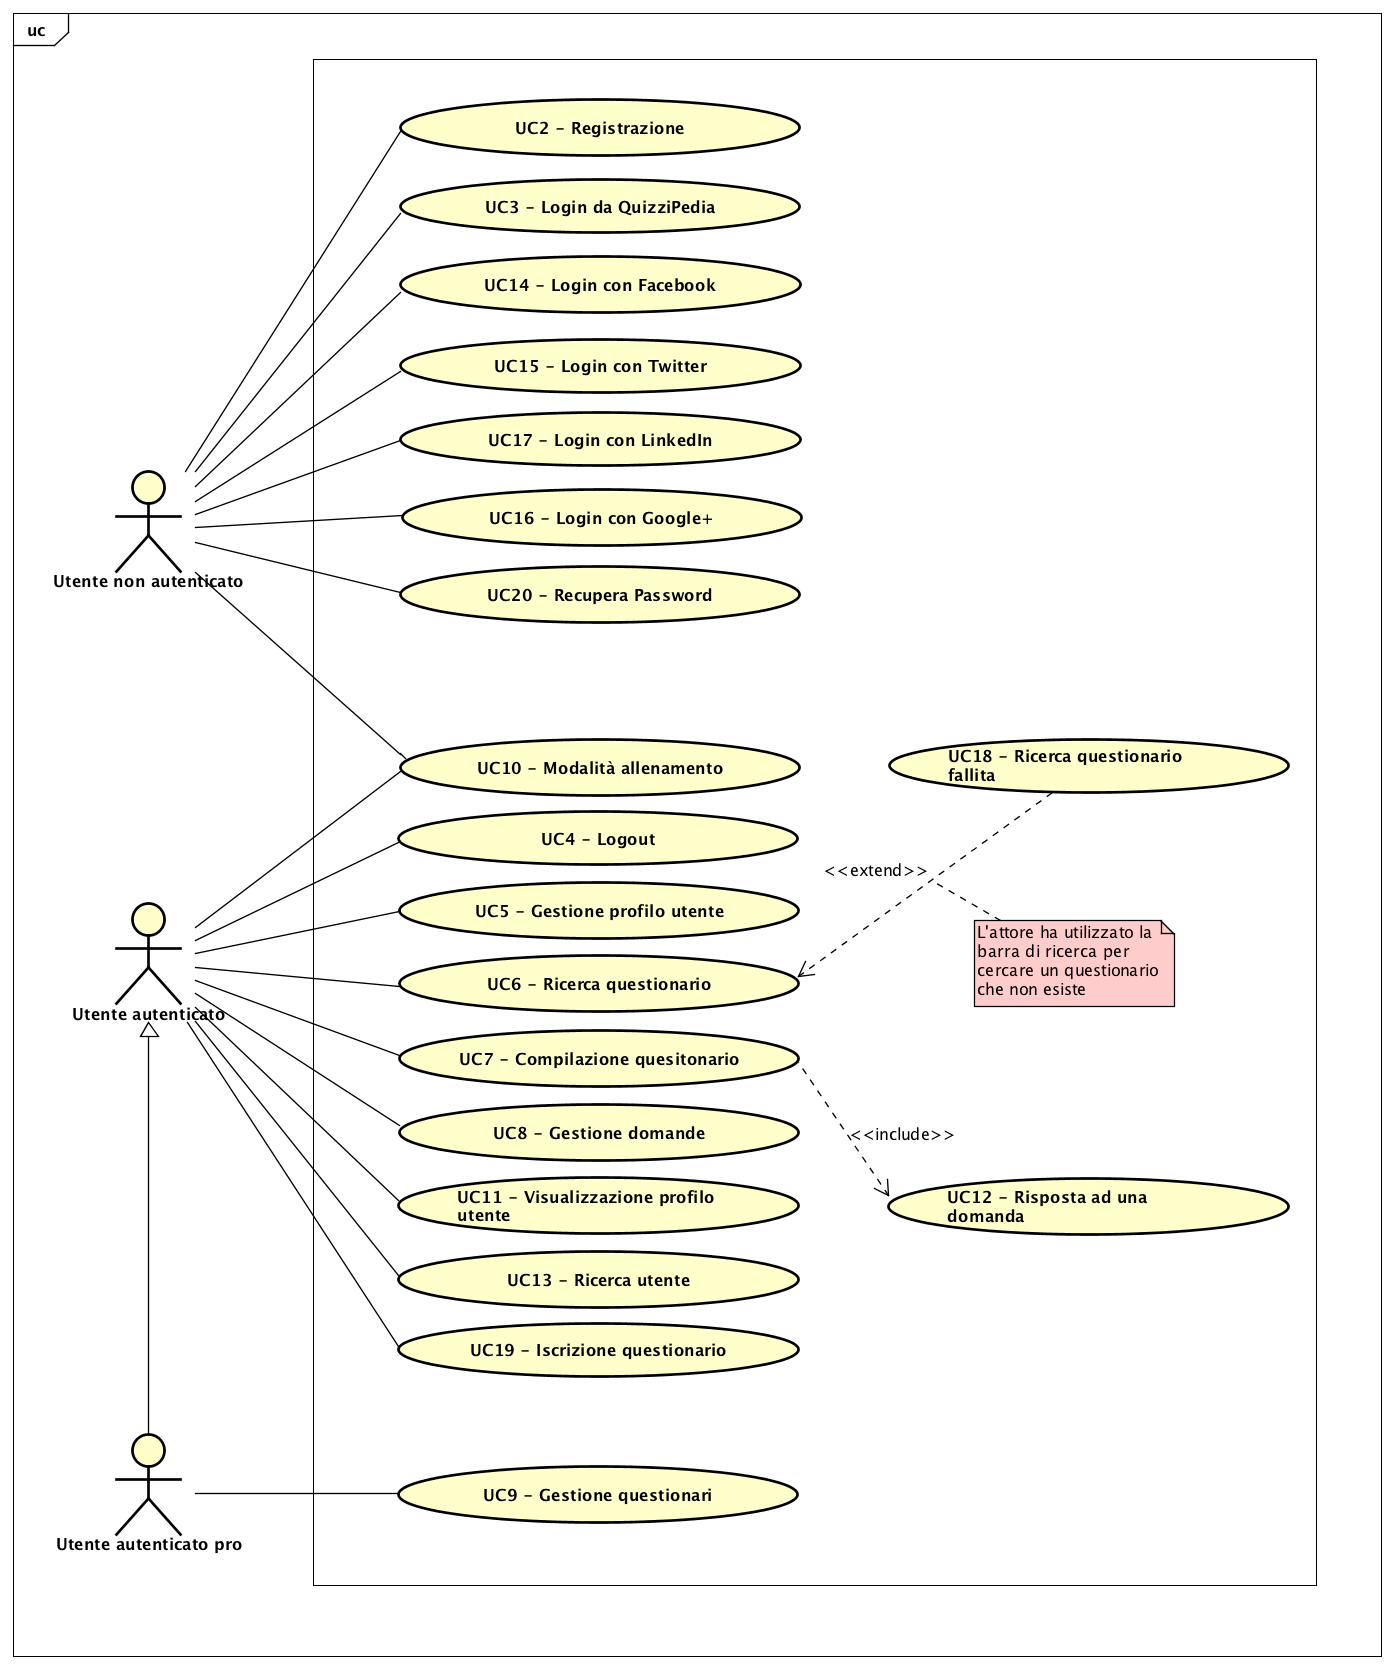
\includegraphics[scale=0.45]{UML/UC1.png}
	\caption{UC1: Scenario principale}
\end{figure}
\FloatBarrier
\begin{itemize}
\item\textbf{Attori}: utente non autenticato, utente autenticato, utente autenticato pro;
\item\textbf{Descrizione}: nella schermata principale un utente non autenticato può autenticarsi tramite l'apposito form di login oppure registrarsi.\\
L'utente autenticato può:
\begin{itemize}
\item Effettuare il logout;
\item Gestire il proprio profilo: modificare il proprio nome, cognome, username, foto/immagine profilo, indirizzo e-mail, password, tipologia di account oppure eliminare il proprio account;
\item Ricercare e iscriversi a questionari: cercare tramite una barra di ricerca i questionari esistenti e iscriversi a questi;
\item Compilare un questionario, se l'autore di questo ha confermato l'iscrizione;
\item Gestire le domande: inserire nuove domande nel sistema oppure modificarne una da lui creata;
\item Visualizzare il profilo utente: visualizzare la cronologia dei questionari svolti, le statistiche per ogni questionario fatto e la lista dei questionari a cui è stato abilitato;
\item Ricercare un utente: ricercare un utente tra tutti quelli che sono iscritti al sistema e visualizzarne il profilo.
\end{itemize}

L'utente autenticato pro può, oltre a svolgere tutte le operazioni dell'utente autenticato, creare questionari oppure modificare o eliminare un questionario da lui creato. Può inoltre gestire la lista di iscrizione e accettare o rifiutare un iscritto.
\\ Infine ogni tipologia di utente descritta precedentemente può usufruire della modalità allenamento, rispondendo a domande, proposte dinamicamente dal sistema, su un argomento scelto;
\item\textbf{Precondizione}: il sistema è avviato e mostra la pagina iniziale dell'applicazione;
\item\textbf{Postcondizione}: il sistema ha ricevuto tutte le informazioni dall'utente sulle operazioni che vuole eseguire;
\item\textbf{Scenario principale}:
\begin{itemize}
\item L'utente non autenticato può registrarsi all'applicazione (UC2);
\item L'utente non autenticato può eseguire il login da \progetto (UC3);
\item L'utente autenticato e l'utente autenticato pro possono eseguire il logout dall'applicazione (UC4); 
\item L'utente autenticato e l'utente autenticato pro possono gestire il proprio profilo utente (UC5);
\item L'utente autenticato e l'utente autenticato pro possono ricercare e iscriversi a questionari (UC6);
\item L'utente autenticato e l'utente autenticato pro possono compilare un questionario selezionato (UC7);
\item L'utente autenticato e l'utente autenticato pro possono gestire le domande (UC8);
\item L'utente autenticato pro può gestire i questionari (UC9);
\item L'attore può fare la modalità allenamento (UC10);
\item L'utente autenticato e l'utente autenticato pro possono visualizzare il proprio profilo personale (UC11);
\item L'utente autenticato e l'utente autenticato pro possono ricercare un utente nel sistema (UC13);
\item L'utente non autenticato può eseguire il login tramite Facebook (UC14);
\item L'utente non autenticato può eseguire il login tramite Twitter (UC15);
\item L'utente non autenticato può eseguire il login tramite Google+ (UC16);
\item L'utente non autenticato può eseguire il login tramite LinkedIn (UC17).
\end{itemize}
\item\textbf{Estensioni}: ricerca questionario fallita (UC18). 
\end{itemize}